\begin{figure}[ht]
\centering
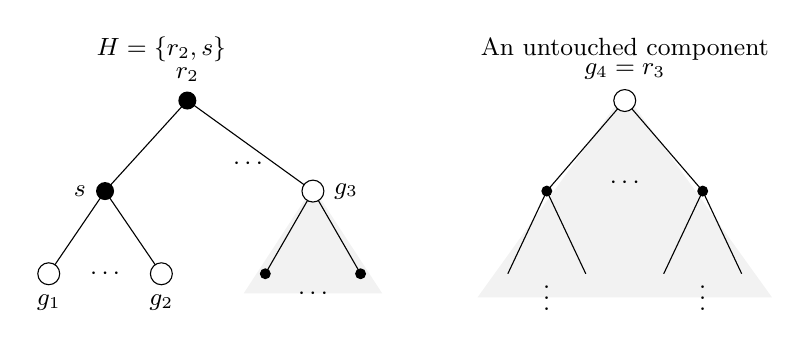
\begin{tikzpicture}[x=1.1cm,y=1cm,
 head/.style={circle,fill=black,inner sep=2.3pt},
 gate/.style={circle,draw,fill=white,inner sep=2.8pt},
 vertex/.style={circle,fill=black,inner sep=1.4pt},font=\small]
\fill[black!5] (1.4,1.1)--(.6,-.25)--(2.2,-.25)--cycle;
\fill[black!5] (5,2.3)--(3.3,-.3)--(6.7,-.3)--cycle;
\draw (-.05,2.2)--(-1,1.05)--(-1.65,0);
\draw (-1,1.05)--(-.35,0);
\draw (-.05,2.2)--(1.4,1.05);
\draw (1.4,1.05)--(.85,0);
\draw (1.4,1.05)--(1.95,0);
\node[head,label=above:$r_2$] at (-.05,2.2) {};
\node[head,label=left:$s$] at (-1,1.05) {};
\node[gate,label=below:$g_1$] at (-1.65,0) {};
\node[gate,label=below:$g_2$] at (-.35,0) {};
\node[gate,label=right:$g_3$] at (1.4,1.05) {};
\node[vertex] at (.85,0) {};
\node[vertex] at (1.95,0) {};
\node at (-1,.0) {$\cdots$};
\node at (.65,1.4) {$\cdots$};
\node at (1.4,-.25) {$\cdots$};
\node at (-.35,2.85) {$H=\{r_2,s\}$};
\draw (5,2.2)--(4.1,1.05)--(3.65,0);
\draw (4.1,1.05)--(4.55,0);
\draw (5,2.2)--(5.9,1.05)--(5.45,0);
\draw (5.9,1.05)--(6.35,0);
\node[gate,label=above:{$g_4=r_3$}] at (5,2.2) {};
\node[vertex] at (4.1,1.05) {};
\node[vertex] at (5.9,1.05) {};
\node at (5,1.15) {$\cdots$};
\node at (4.1,-.2) {$\vdots$};
\node at (5.9,-.2) {$\vdots$};
\node at (5,2.85) {An untouched component};
\end{tikzpicture}
\caption{A finite ancestor-closed head and some of its gates.  Black
large nodes belong to $H$; circled nodes are gates.  Shading indicates
two complementary descendant cones.  Only finitely many of the
countably many branches are drawn.  In particular an untouched
component begins with a gate at its root.}\label{fig:forest-gates}
\end{figure}
